%----------------------------------------------------------------------------------------
%	PACKAGES AND OTHER DOCUMENT CONFIGURATIONS
%----------------------------------------------------------------------------------------

\documentclass[paper=a4,fontsize=12pt]{article}

\usepackage{fancyhdr} % Required for custom headers
\usepackage{lastpage} % Required to determine the last page for the footer
\usepackage{extramarks} % Required for headers and footers
\usepackage[usenames,dvipsnames]{color} % Required for custom colors
\usepackage{graphicx} % Required to insert images
\usepackage{listings} % Required for insertion of code
\usepackage{courier} % Required for the courier font
\usepackage{amssymb}
\usepackage{amsmath,amsfonts,amsthm} % Math packages into the template
\usepackage{listings}
\usepackage[utf8]{inputenc}
\usepackage{float}
\usepackage{caption}
\usepackage{subcaption}


% Default fixed font does not support bold face
\DeclareFixedFont{\ttb}{T1}{txtt}{bx}{n}{12} % for bold
\DeclareFixedFont{\ttm}{T1}{txtt}{m}{n}{12}% for normal

% Declare colour
\usepackage{color}
\definecolor{codebg}{RGB}{250,250,250}
\definecolor{codeframe}{RGB}{230,230,230}
\definecolor{deepblue}{rgb}{0,0,0.5}
\definecolor{deepred}{rgb}{0.6,0,0}
\definecolor{deepgreen}{rgb}{0,0.5,0}


% Margins
\topmargin=-0.45in
\evensidemargin=0in
\oddsidemargin=0in
\textwidth=6.5in
\textheight=9.0in
\headsep=0.25in

\lstloadlanguages{Python}
\lstset{ %
language=Python,
backgroundcolor=\color{codebg},
basicstyle=\ttm,
otherkeywords={self}, 
keywordstyle=\ttb\color{deepblue},
stringstyle=\color{deepgreen},
frame=tb,
rulecolor=\color{codeframe},
showstringspaces=false,
breaklines=true
}


\newcommand{\pythonscript}[3]{
\begin{small}
\lstinputlisting[firstline=#2,lastline=#3]{#1.py}
\end{small}
}


%----------------------------------------------------------------------------------------

\title{Comparing Regularisation Techniques for Logistic Regression}
\author{Sujith Padaru \& Pashupati Hegde}
\date{\today}

%----------------------------------------------------------------------------------------

\begin{document}
\maketitle
\rule{\linewidth}{0.5pt}

\section{Abstract}
In this report we tackle the problem of predicting rating for Yelp reviews based on the bag of words representation of the review. The problem is designed as classification task by considering reviews with $\geq 4$ ratings as 'class 1' and $< 4$ as 'class 0'. We incorporate logistic regression model approach for classification and study the impact of L1 \& L2 regularisation in various dimensional settings. In addition to on low-dimensional dataset with original 50 features, we create another high-dimensional dataset with around 1275 features with 2-way feature interactions. It is shown that in low-dimensions, regularisation doesn't give much improvement over the standard regression. In high-dimensional data L1 regularisation for feature selection followed by model training using L2 regularisation gives the best results as compared to L1 \& L2 in isolation.


\section{Introduction}
Logistic is regression is one of the novel parametric techniques used in case of classification problems. But it is well known that logistic regression overfits in case of high-dimensional data where there are many irrelevant features. L1 \& L2 are the two regularisation techniques that induce penalty on the higher weight values and in turn make the model less prone to overfitting. It is also suggested that L1 regularisation performs the best for feature selection by introducing sparse weight matrix where as L2 regularisation works better for predicting using the model. Here we study both the methods on low-dimensional and high-dimensional settings.



\section{Method}
\subsection{Logistic Regression$^{[1]}$}
Logistic Regression is a parametric method of classification used for predicting binary dependent target variables. Probability or Odds of "success" is modeled as a logit transformation of linear combination of the features.\\
For a data with N records with m dimensions, logistic regression model is defined as:
\begin{align*}
\begin{split}
\pi_i = Pr(Y_i=1|X) = \frac{e^W}{1+e^W}\\
W = \sum_{j=1}^{m} (\beta_j x_j)
\end{split}
\end{align*}

Logit transformation of $\pi$ is given as: 
\begin{align*}
\begin{split}
logit(\pi_i) = log(\frac{\pi_i}{1-\pi_i})
&= \sum_{j=1}^{m} (\beta_j x_j)
\end{split}
\end{align*}

Parameters of the model $\beta$ are estimated from Maximum Likelihood Estimation method, that is the values of $\beta_j$ that maximizes:
\begin{align*}
\begin{split}
L(X|\beta) = \prod_{i=1}^{N} \pi_i^{y_i} (1-\pi_i)^{n_i - y_i}  
\end{split}
\end{align*}
Gradient descent method is used for MLE where the loss function is defined as:
\begin{align*}
\begin{split}
Loss = \sum_{i=1}^{N} (y_i log(p_i) + (1-y_i)log(1-p_i)
\end{split}
\end{align*}


\subsection{Regularisation}
Regularisation is a technique to prevent to over-fitting in Machine Learning. A regularisation term is added to the Loss function in order to penalize higher values for weights.\\
L1 regularisation specifically penalises the absolute value of weights and produces sparse weight matrix in case of high-dimensional data. 
\begin{align*}
\begin{split}
Loss_{L1} = \sum_{i=1}^{N} (y_i log(p_i) + (1-y_i)log(1-p_i) + \lambda \sum_{j=1}^{M} |w_j|
\end{split}
\end{align*}
L2 regularisation penalises the squared value of weights and reduces the chances of overfitting in case of high-dimensional noisy data.
\begin{align*}
\begin{split}
Loss_{L2} = \sum_{i=1}^{N} (y_i log(p_i) + (1-y_i)log(1-p_i) + \lambda \sum_{j=1}^{M} w_j^2
\end{split}
\end{align*}

Where $\lambda$ called as regularisation coefficient is a hyperparamter and is tuned usually through cross validation technique.

\subsection{Modeling}
It is generally seen that the L1 regularisation generates sparse weight matrix and hence can be a choice for feature selection in case of high-dimensional data where there could be many irrelevant features. L2 regularisation on the other hand is rotationally invariant and provides better model for prediction.\\



\section{Experiments}
\subsection{Feature Engineering}
The Yelp dataset contains 5000 Yelp reviews with word counts of 50 keywords as features and the rating as a binary target feature of 1's and 0's representing a rating of $\geq 4$ and $< 4$ respectively. A dataset of 1000 additional reviews was used for testing the best model. \\

As a part of feature engineering, in addition to the original features, two-way interaction features were added considering all the possible feature combinations. Two-way interaction of features $x \& y$ is computed as product of features $(x*y)$. Thus the 50 base features in the data lead to 1225 additional combinations of interaction features. Here onwards we refer to dataset with 50 features as low-dimensional data and the one with additional 1225 features (total of 1775 features) as high-dimensional data.  

\subsection{Model Implementation}
Logistic Regression with gradient descent solver was implemented in Python. In addition, L2 regularisation technique was also implemented. Since L1 regularisation doesn't have an analytical solution form, standard library implementation from $scikit-learn$ module was used.\\

In the project we study the effect of L1 and L2 regularisation techniques in case of low-dimensional and high-dimensional data for different values of regularisation coefficients. \\

A modeling choice of using L1 regularisation for feature selection and using L2 regularisation for prediction is also studied for the pertinent data and shown to perform better than isolated L1 and L2 regularisation models in case of high-dimensional data.


\subsection{Model Validation}
Training data of 5000 rows was split into $3-$folds and cross validation technique was used for model validation and parameter tuning. Overall classification accuracy and ROC area under the curve metrics were used to the model performance. 

\section{Results}
\subsection{Low-dimensional data with original 50 features}
Standard logistic regression was performed without any regularisation on the low-dimensional data, it gives an accuracy of 0.709 and AUC of 0.750.
\begin{figure}[H]
\centering
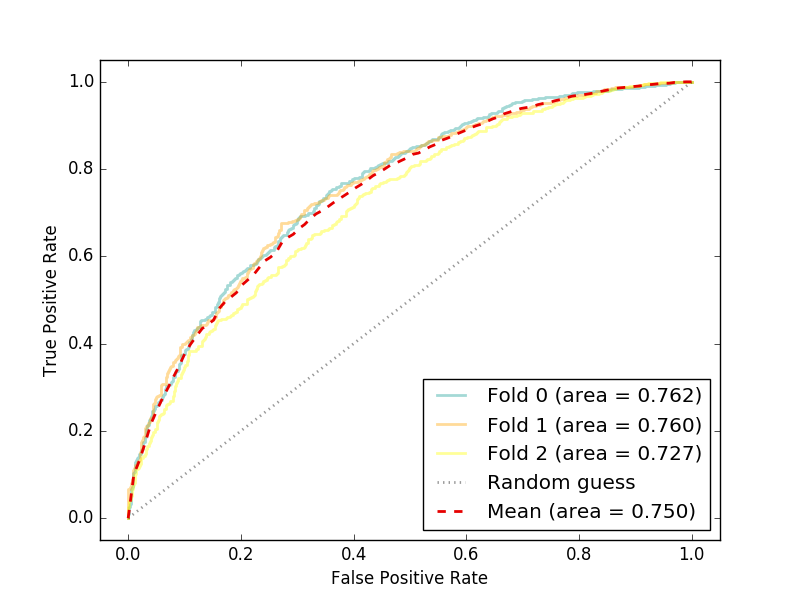
\includegraphics[width=0.5\linewidth]{00_noregularisation_of}
\caption{Cross validation ROC for logistic regression without regularisation}
\end{figure}

Regularisation was added to the above model using both L1 and L2 regularisations for varying values of regularisation coefficients ($\lambda$) between $(10^{-2},10^6)$. Figure 2 below compares the charts for L1 and L2 regularisations. It can be seen that the weights for different 50 features for L1 taper off zero earlier than L2 for same $\lambda$ value.

\begin{figure}[H]
\centering
\begin{subfigure}{.5\textwidth}
  \centering
  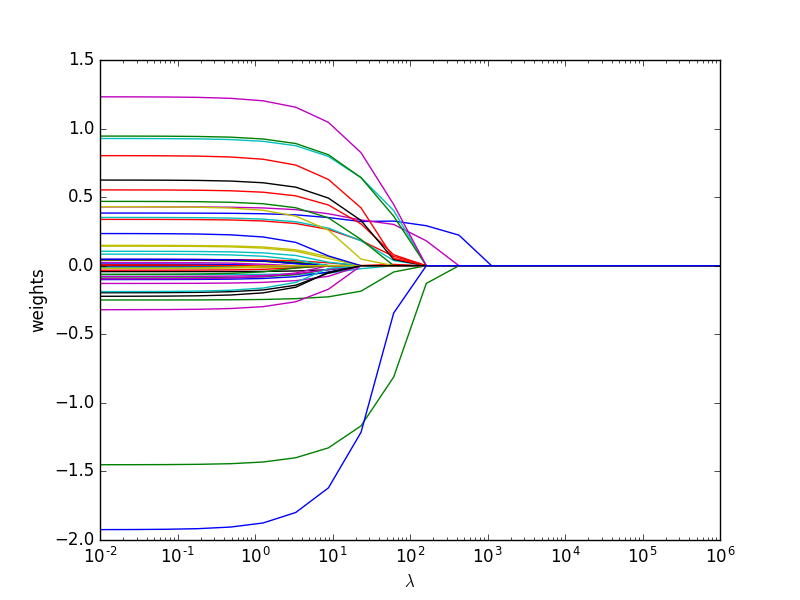
\includegraphics[width=1\linewidth]{01_L1regularisation_of_wm}
  \caption{L1 regularisation}
  \label{fig:sub1}
\end{subfigure}%
\begin{subfigure}{.5\textwidth}
  \centering
  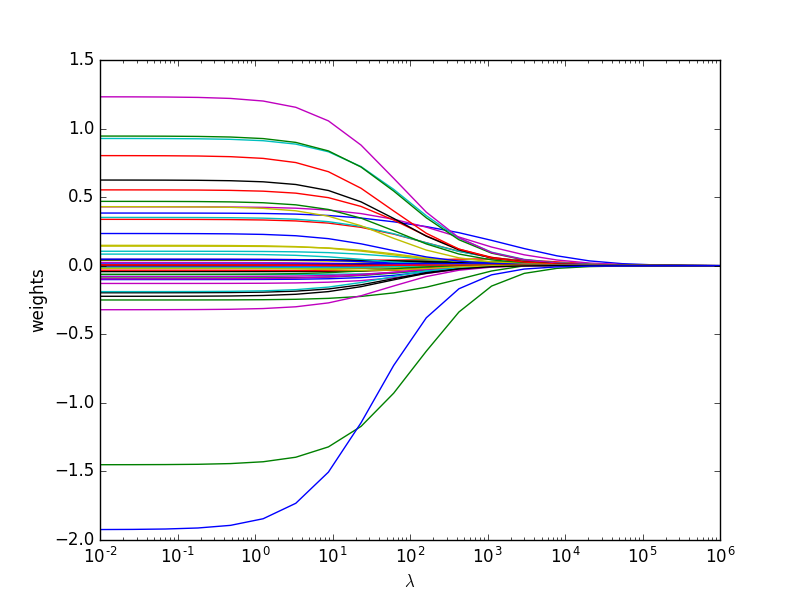
\includegraphics[width=1\linewidth]{02_L2regularisation_of_wm}
  \caption{L2 regularisation}
  \label{fig:sub2}
\end{subfigure}
\caption{Change in weights for varying $\lambda$}
\label{fig:test}
\end{figure}

Figure 3 compares the ROC charts for L1 and L2 regularisations. Best value for $\lambda$ was selected from cross validation. It can be seen that both the regularisation settings perform similar to the model without any regularisation.


\begin{figure}[H]
\centering
\begin{subfigure}{.5\textwidth}
  \centering
  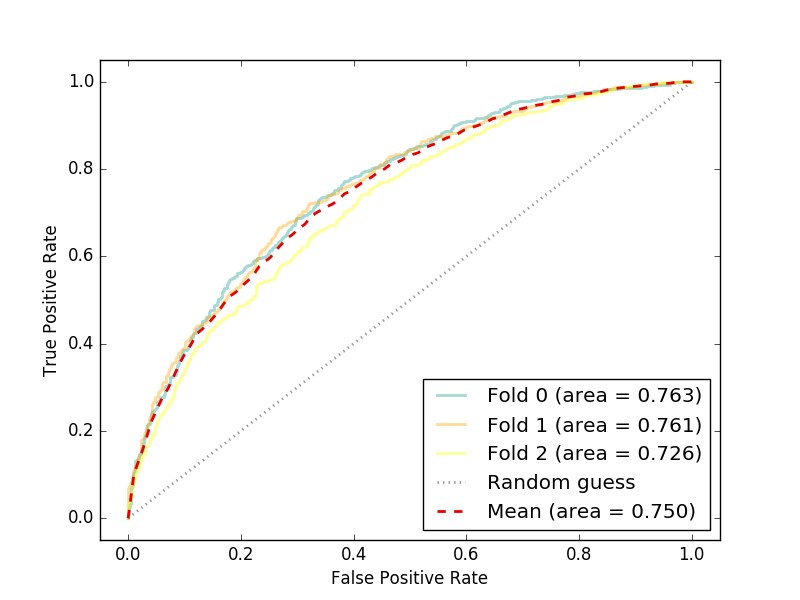
\includegraphics[width=1\linewidth]{01_L1regularisation_of}
  \caption{L1 regularisation}
  \label{fig:sub1}
\end{subfigure}%
\begin{subfigure}{.5\textwidth}
  \centering
  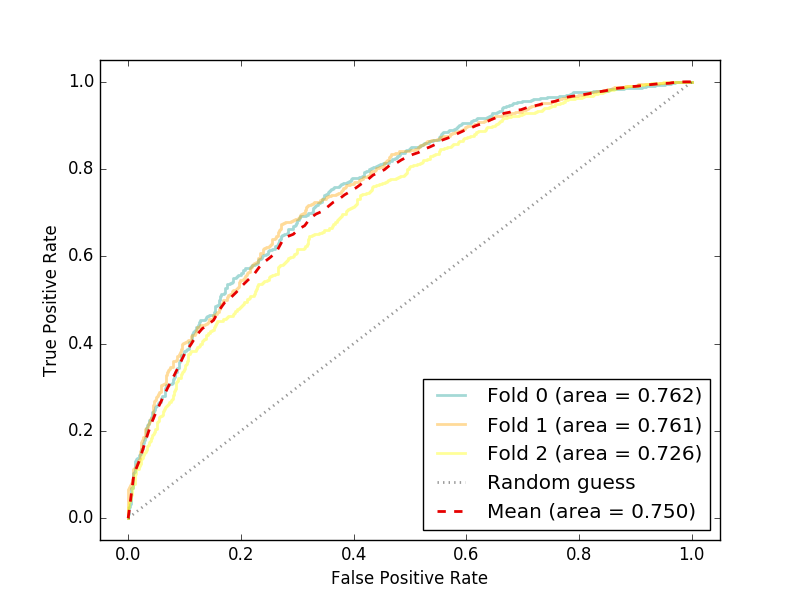
\includegraphics[width=1\linewidth]{02_L2regularisation_of}
  \caption{L2 regularisation}
  \label{fig:sub2}
\end{subfigure}
\caption{Cross validation ROC for logistic regression with regularisation}
\label{fig:test}
\end{figure}


Following table summarises the results for various approaches. It can be seen that all the three models perform almost similarly. It can be seen that in case of low-dimensional data, for the given example there are not many irrelevant features hence regularisation doesn't bear much improvement in the model performance. \\

\begin{center}
\large
\begin{tabular}{ | c | c | c | } 
\hline
Model & Accuracy (+/- 2$\sigma$) & AUC (+/- 2$\sigma$) \\ 
\hline
Logistic without regularisation & 0.709 (+/- 0.03) & 0.750 (+/- 0.03) \\ 
Logistic with L1 regularisation & 0.710 (+/- 0.02) & 0.751 (+/- 0.03) \\ 
Logistic with L2 regularisation & 0.708 (+/- 0.03) & 0.750 (+/- 0.03) \\ 
\hline
\end{tabular}
\end{center}


\clearpage
\subsection{High-dimensional data with 1277 features}
Interaction features were added to the above datasets anticipating an improve in model performance. Firstly, standard logistic regression was performed without any regularisation on the high-dimensional data. Due to presence of irrelevant features, without regularisation, logistic regression overfits and the model performs worse than that on the original 50 features.
\begin{figure}[H]
\centering
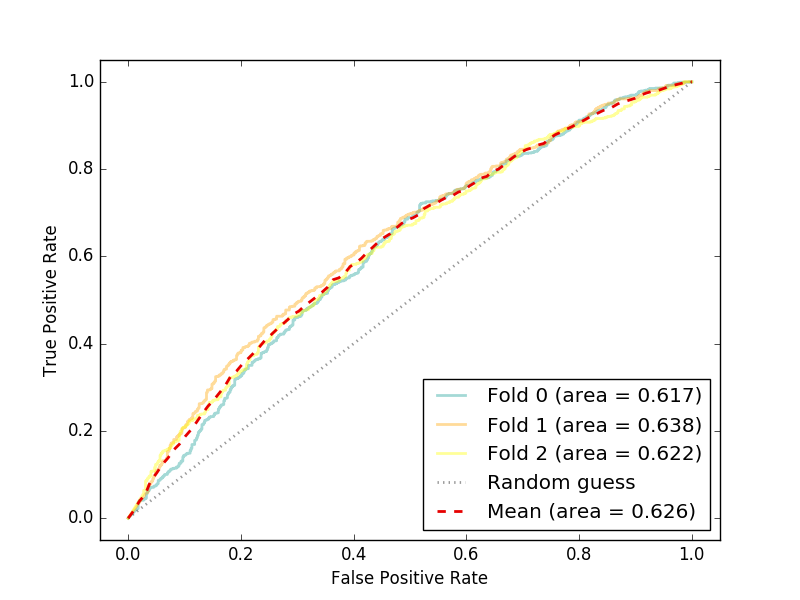
\includegraphics[width=0.5\linewidth]{04_noregularisation_hf}
\caption{Cross validation ROC for logistic regression without regularisation}
\end{figure}

Regularisation was added to the above model using both L1 and L2 regularisations for varying values of regularisation coefficients ($\lambda$) between $(10^{-2},10^6)$. Figure 5 below compares the charts for L1 and L2 regularisations. It can be seen that the weights for different 1277 features for L1 generates sparse weights as compared to L2.

\begin{figure}[H]
\centering
\begin{subfigure}{.5\textwidth}
  \centering
  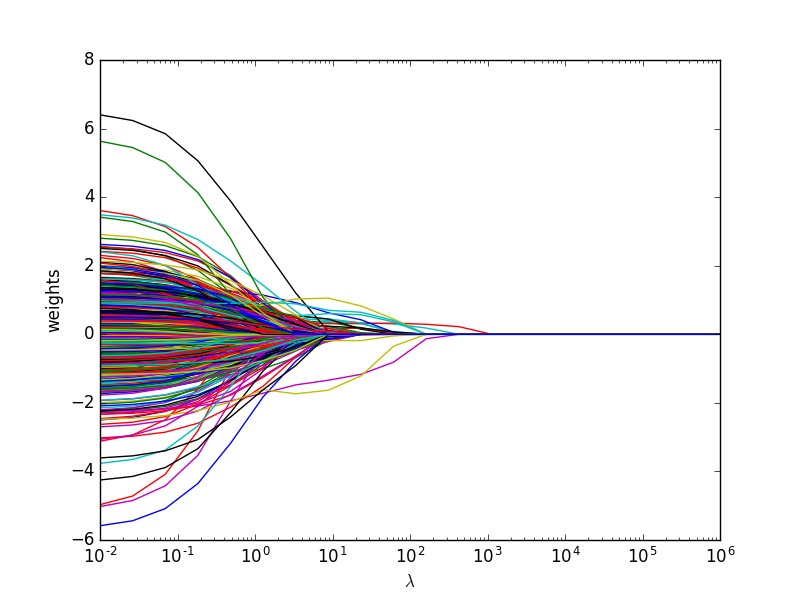
\includegraphics[width=1\linewidth]{05_L1regularisation_hf_wm}
  \caption{L1 regularisation}
  \label{fig:sub1}
\end{subfigure}%
\begin{subfigure}{.5\textwidth}
  \centering
  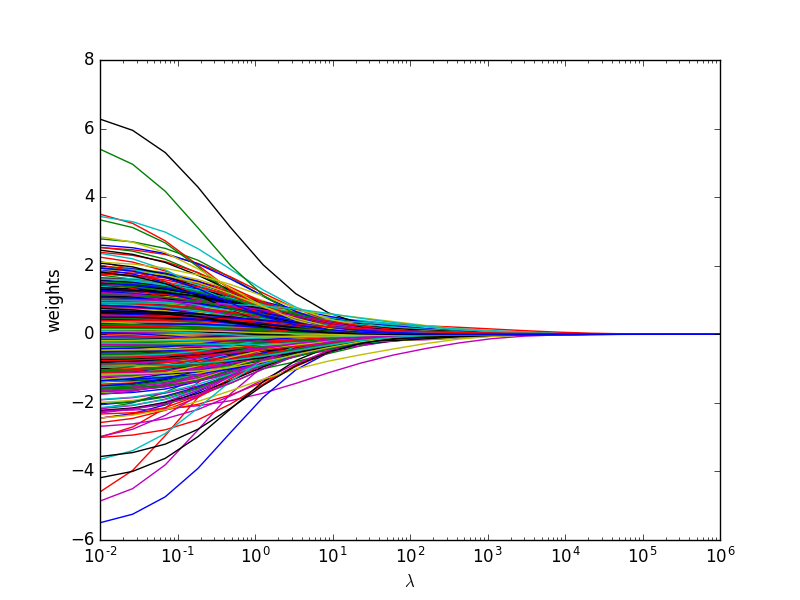
\includegraphics[width=1\linewidth]{06_L2regularisation_hf_wm}
  \caption{L2 regularisation}
  \label{fig:sub2}
\end{subfigure}
\caption{Change in weights for varying $\lambda$}
\label{fig:test}
\end{figure}

Figure 6 compares the ROC charts for L1 and L2 regularisations. Best value for $\lambda$ was selected from cross validation. It can be seen that both the regularisation settings perform almost similarly. It can also be seen that both these models perform better than the one without regularisation.


\begin{figure}[H]
\centering
\begin{subfigure}{.5\textwidth}
  \centering
  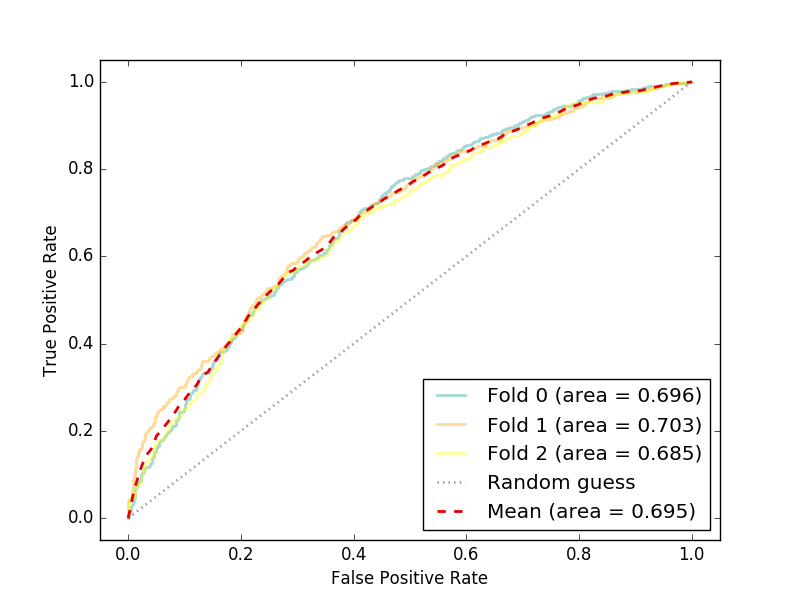
\includegraphics[width=1\linewidth]{05_L1regularisation_hf}
  \caption{L1 regularisation}
  \label{fig:sub1}
\end{subfigure}%
\begin{subfigure}{.5\textwidth}
  \centering
  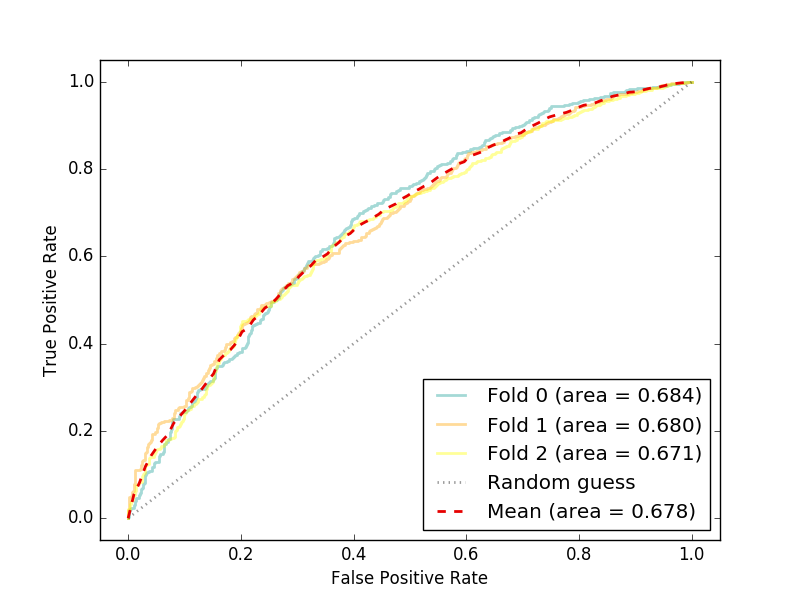
\includegraphics[width=1\linewidth]{06_L2regularisation_hf}
  \caption{L2 regularisation}
  \label{fig:sub2}
\end{subfigure}
\caption{Cross validation ROC for logistic regression with regularisation}
\label{fig:test}
\end{figure}

But with additional interaction features in high-dimensional data, even after regularisation the prediction performance is not better than the model on original 50 features.


\subsection{High-dimensional data with L1 for feature selection and L2 for prediction}
Upon considering the notion that L1 produces sparse weight matrix and L2 performs better for prediction, a new approach was followed with performing L1 on the high-dimensional data for feature selection to arrive at non-zero weight features. Thus filtered were then used to build a new L2 regularised model for prediction. \\

Figure 7 (a) shows the performance of the above model for different values of regularisation parameters of L1 \& L2. It can be seen that for a specific range of $\lambda_{L1}$ the above setting gives best results for a wide range of $\lambda_{L2}$ values.
Figure 7 (b) shows the cross validation ROC for best parameters $\lambda_{L1}$ \& $\lambda_{L2}$.


\begin{figure}[H]
\centering
\begin{subfigure}{.5\textwidth}
  \centering
  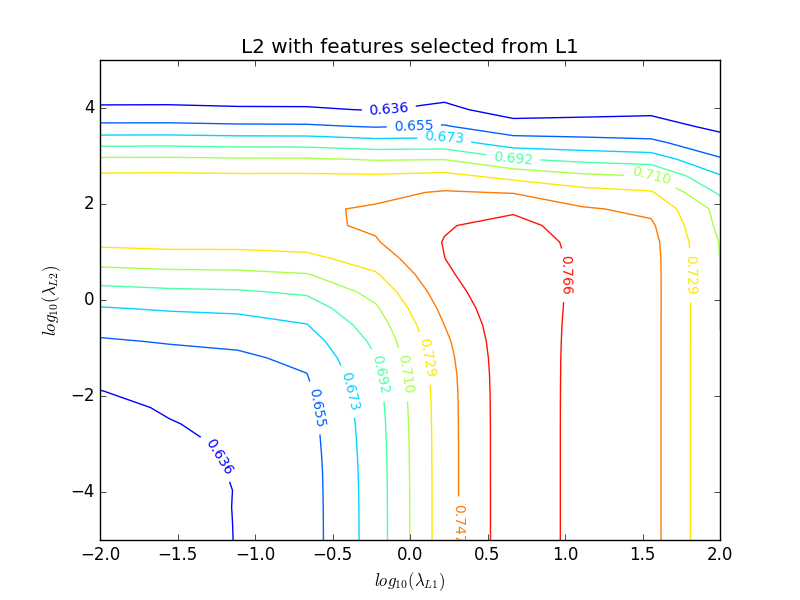
\includegraphics[width=1\linewidth]{contourplot_auc}
  \caption{AUC for different $\lambda_{L1}$ \& $\lambda_{L2}$}
  \label{fig:sub1}
\end{subfigure}%
\begin{subfigure}{.5\textwidth}
  \centering
  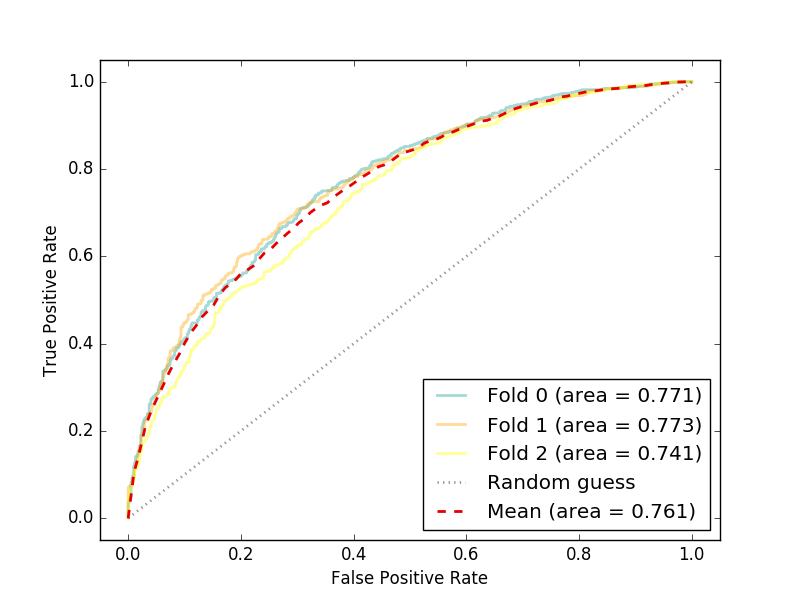
\includegraphics[width=1\linewidth]{07_L2regularisation_L1selectedf}
  \caption{ROC performance}
  \label{fig:sub2}
\end{subfigure}
\caption{Model with L1 feature selection \& L2 prediction}
\label{fig:test}
\end{figure}


Following table summarises the results for various approaches on high-dimensional data. It can be seen stand alone, L1 \& L2 models perform worse than the 50-feature models. But upon using the L1 for feature selection and L2 for prediction model accuracy improves more than rest of the models.

\begin{center}
\large
\begin{tabular}{ | c | c | c | } 
\hline
Model & Accuracy (+/- 2$\sigma$) & AUC (+/- 2$\sigma$) \\ 
\hline
Logistic without regularisation & 0.630 (+/- 0.03) & 0.643 (+/- 0.04)\\ 
Logistic with L1 regularisation & 0.672 (+/- 0.03) & 0.698 (+/- 0.03) \\ 
Logistic with L2 regularisation & 0.657 (+/- 0.03) & 0.681 (+/- 0.03) \\ 
L2 prediction with L1 regularisation & 0.720 (+/- 0.02) & 0.764 (+/- 0.04) \\ 
\hline
\end{tabular}
\end{center}


\subsection{Performance on test data}
Running the best performing model on the test data gives an accuracy of 0.7169 and auc score of 0.7488.


\section{Conclusion}
In low-dimensional data, there are not many irrelevant features and hence regularisation doe not bear much improvement on the model performance. It is shown that logistic regression without any regularisation performs almost same as L1 and L2 regularised models.\\

In high-dimensional data by adding interaction features introduces many irrelevant features to the data. Logistic regression without any regularisation overfits the data and doesn't perform well. L1 performs better than L2 regularisation as it does inherent feature selection in the model. L2 regularisation performance is lower than that of L1.\\ 

It could be a reason that the amount sample data required to learn "well" for L1 regularisation grows $logarithamically$ in number of irrelevant features where in case of L2 it grows $linearly$ in worst case $^{[2]}$.\\

Lastly, it is also seen that L2, being a better regulariser as compared L1 for prediction, performs the best on subset of features in high-dimensional data, with features selected using L1 regularisation.


\section{Reference}
$^{[1]}$ https://onlinecourses.science.psu.edu/stat504/node/150 \\
$^{[2]}$ Feature selection, L1 vs. L2 regularisation, and rotational invariance by Andrew NG.


\clearpage
\section{Appendices}
\pythonscript{LogisticRegression}{1}{151}



\end{document}